\documentclass[12pt,a4paper]{scrartcl}
\usepackage[utf8]{inputenc}
\usepackage{mathtools}
\usepackage[english,russian]{babel}
\usepackage{graphicx}
\usepackage{multicol}

\begin{document}
	\begin{titlepage}
		\begin{center}
			
			\vspace{0.5cm}
			
			НОВОСИБИРСКИЙ ГОСУДАРСТВЕННЫЙ УНИВЕРСИТЕТ
			\vspace{0.25cm}
			
			Механико-математический факультет
			
			Кафедра: Математика и компьютерные науки
			\vfill
			
			
			Тлепбергенова Дарья Дулатовна
			\vfill
			
			\textsc{Отчет по вычислительному практикуму}\\[5mm]
			
			{\LARGE Решение уравнения переноса\\
				с помощью неявной схемы бегущего счета.\\
				Вариант 12.\\[2mm]}
			\bigskip
			
			3 курс, группа 16121
		\end{center}
		\vfill
		\newlength{\ML}
		\settowidth{\ML}{«\underline{\hspace{0.7cm}}» \underline{\hspace{2cm}}}
		\hfill\begin{minipage}{0.4\textwidth}
			Преподаватель:\\
			Махоткин Олег Александрович
		\end{minipage}%
		\bigskip
		
		\vfill
		\begin{center}
			Новосибирск, 2018 г.
		\end{center}
	\end{titlepage}
	
	%----------------------------------------------------------------------------
	\newpage
	\section{Постановка задачи.}
	Дано уравнение переноса в виде:
	\begin{align}\label{main}
	\begin{cases}
	\frac{\partial u}{\partial t}+C(x,t) \frac{\partial u}{\partial x}=0, \\
	0\le x \le 1, 0\le t \le1 \\        
	u(x,0)=\varphi_{0}(x) \\
	\end{cases}
	\end{align}
	
	С помощью неявной схемы бегущего счета:
	\begin{align}\label{method}
	\frac{u^{j+1}_{k}-u^{j}_k}{\tau}+C\frac{u^{j+1}_{k}-u^{j+1}_{k-1}}{h}=0, \text{при } C \ge 0 \\
	\frac{u^{j+1}_{k}-u^{j}_k}{\tau}-C\frac{u^{j+1}_{k}-u^{j+1}_{k-1}}{h}=0, \text{при } C < 0 
	\end{align}
	
	Для:
	\begin{align*}
	\begin{cases}
	u(x,t) = -(t-0.3)^3+cos(\pi x)+2 \pi x, \\
	\varphi_{0}(x) = cos(\pi x)+0.027+2 \pi x, \\
	u(0,t) = t \\
	C(x,t) = \frac{3(t-0.3)^2}{2 \pi - \pi sin(\pi x)},\\
	\end{cases}
	\end{align*}
	Выполнить следующие пункты:
	\begin{enumerate}
		\item Исследовать данную схему на точность и устойчивость.
		\item Найти решение уравнения переноса в узлах сетки.
		\item Вывести на экран графики приближенного и точного решения для значений t от 0 до 1 с шагом 0.1 и для $x = 0.5$.
	\end{enumerate}
	%----------------------------------------------------------------------------
	\section{Описание вычислительного метода.}
	Перейдем к дискретной постановке задачи: разобьем наши промежутки по $x$ и по $t$ на $N_x$ и $N_t$ равных частей соответственно. Тогда задача \eqref{main} с учетом \eqref{method}:
	
	\begin{align}
	\begin{cases}
	\frac{u^{j+1}_{k}-u^{j}_k}{\tau}+C^{j+1}_{k}\frac{u^{j+1}_{k}-u^{j+1}_{k-1}}{h}=0, \text{при } C^{j+1}_{k} \ge 0 \\
	\frac{u^{j+1}_{k}-u^{j}_k}{\tau}-C^{j+1}_{k}\frac{u^{j+1}_{k}-u^{j+1}_{k-1}}{h}=0, \text{при } C^{j+1}_{k} < 0 \\
	\Bigl\{x_k = k h $ : $ h = \frac {1}{N_x}, k = 0 ..N_x\Bigr\}\\
	\Bigl\{t_j = j \tau $ : $ \tau =\frac {1}{N_t}, j = 0 ..N_t \Bigr\}\\ \label{dis}
	u^{0}_k = \varphi_{0}(x_k) \\
	u^{j}_0 = u_0(t_j) \\
	\end{cases}
	\end{align}
	
	данный метод соответсвует графической схеме:
	\begin{figure}[h]
		\centering
		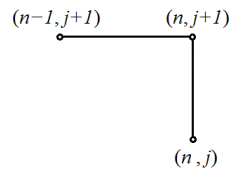
\includegraphics{method.png}
		\caption{Шаблон для схемы бегущего счета}
	\end{figure}
	%----------------------------------------------------------------------------
	\section{Исследование данной схемы на точность и устойчивость.}    
	\subsection{Погрешность апроксимации:}
	В данном случае разностный оператор $L_{h \tau}$ будет иметь вид:
	\[
	L_{h \tau}u = \frac{u^{j+1}_{k}-u^{j}_k}{\tau}+C^{j+1}_{k}\frac{u^{j+1}_{k}-u^{j+1}_{k-1}}{h}
	\]
	и выражение $L_{h \tau}u$ апроксимирует $Lu$ в точке $(x_k,t_{j+1})$ с погрешностью $O(\tau + h)$:
	\[
	L_{h \tau}u = (	\frac{\partial u}{\partial t}+C(x,t) \frac{\partial u}{\partial x})\Bigm|_{x_k,t_{j+1}}+O(\tau+h)
	\]
	
	\subsection{Погрешность решения:}
	Погрешность $\xi^j_k $ решения разностной схемы \eqref{method}, обусловленная погрешностью начальных данных, будет удовлетворять уравнению
	\begin{align*}
	&L_{\tau,h} \xi^{\tau,h} = \psi^{\tau,h}\\
	&\xi^{j}_{k} = u^{j}_k - u(x_k,t_j) \\
	&\xi^{j+1}_k = \xi^j_k - \frac{c \tau}{h}(\xi^{j+1}_k-\xi^{j+1}_{k-1})
	\end{align*}
	
	Разложим сеточную функцию $\xi^j_k$ в ряд по $e^{iqx_k}$
	\[
	\xi^j_k = \sum_q \xi^j_{k,q}=\sum_q C_q^j e^{iqx_k}   
	\]
	Так как схема \eqref{method} является линейной двухслойной схемой с постоянными коэффициентами, то на слое $(j + 1)$ погрешность будет иметь вид
	\[
	\xi^{j+1}_k = \sum_q \xi^{j+1}_{k,q}=\sum_q \lambda_q C_q^j e^{iqx_k} \text{ где } \lambda_q \text{- множители роста}
	\]
	Введем обозначения $r=\frac{c \tau}{h}$ и $\alpha_q = qh$. Тогда, рассматривая уравнения для каждой гармоники $\xi^{j}_{k,q}$ в отдельности, получаем:
	\[
	\xi^{j+1}_k = \xi^j_k - r(\xi^{j+1}_k-\xi^{j+1}_{k-1})
	\]
	Или, что тоже самое,
	\[
	\lambda_q C_q^j e^{i \alpha_q k} = C_q^j e^{i \alpha_q k}-r(\lambda_q C_q^j e^{i \alpha_q k}-\lambda_q C_q^j e^{i \alpha_q (k-1)})
	\]
	Сокращая на $C_q^j e^{i \alpha_q k}$, и выполнив несколько несложных преобразований, получаем:
	\[
	\frac{\lambda_q -1}{\tau}+c \lambda_q \frac{1-e^{-i \alpha_q}}{h}=0,
	\]
	Откуда получаем:
	\[
	\lambda_q = \frac{1}{1+r-re^{-i \alpha_q}}=\frac{1}{\beta_q}, \text{ где } \beta_q = 1+r-re^{-i \alpha_q}, 
	\]
	Спектр $\lambda_q(\alpha_q)$ оператора перехода со слоя на слой в рассматриваемой задаче представляет собой окружность на комплексной плоскости с центром в точке $1 - r$ и радиусом $|r|$. Так как $\lambda_q(\alpha_q)$ не зависит от $\tau$ явным образом, то спектральное условие устойчивости схемы принимает вид:
	\begin{align} \label{spectr}
	| \lambda_q | \le 1, \forall q. 
	\end{align}
	Следовательно, для того чтобы схема \eqref{method} была устойчивой по начальным данным, необходимо и достаточно, чтобы спектр оператора перехода со слоя на слой полностью содержался в круге единичного радиуса с центром в нуле на комплексной плоскости.
	
	\begin{figure}[h]
		\centering
		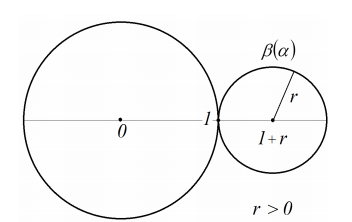
\includegraphics[width=0.3\textwidth]{picture2.png}
		\caption{Спектр оператора перехода со слоя на слой в схеме \eqref{method} при $c \ge 0$, $0 \le r \le 1$}
		\label{pic2}
	\end{figure}
	
	Очевидно, что условие \eqref{spectr} выполняется, если $| \beta_q| \ge 1$. При изменении параметра $\alpha_q$ от минус до плюс бесконечности значения функции $\beta_q(\alpha_q)$ пробегают окружность радиуса $|r|$ с центром в точке $1 + r$ на комплексной плоскости.
	
	При $c > 0$ параметр $r$ также положителен. Следовательно, окружность, заполняемая значениями $\beta_q$, расположена вне единичного круга с центром в начале координат и касается единичной окружности в точке 1 (\eqref{pic2}). Это означает, что $| \beta_q| \ge 1$. при любом соотношении $\tau$ и $h$, то есть при положительном $c$ схема \eqref{method} безусловно устойчива по начальным данным.
	
	\begin{figure}[h]
		\centering
		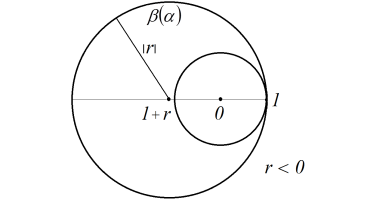
\includegraphics[width=0.3\textwidth]{picture3.png}
		\caption{Спектр оператора перехода со слоя на слой в схеме \eqref{method} при $c \le 0$}
		\label{pic3}
	\end{figure}
	
	Если скорость переноса $c$ отрицательна, то и параметр $r$ отрицателен, и условие $| \beta_q| \ge 1$ устойчивости схемы \eqref{method} будет выполнено при $|r| \ge 1$ (\eqref{pic3}). Следовательно, при $c < 0$ схема \eqref{method} является условно устойчивой по начальным данным, и условие ее устойчивости имеет вид $|c|\tau \ge h$ . 
	
	Но в силу того, что в нашем случае при $c < 0$ мы выбираем зеркальный аналог сахемы, который наоборот безусловно устойчив при $c < 0$ и условно устойчив иначе получаем, что для такой комбинированной схемы имеем безусловную устойчивость на всем промежутке.
	
	Метод гармоник применим только для схем с постоянными коэффициентами. Для исследования на устойчивость разностных схем для уравнений с переменными коэффициентами широко используют прием «замораживания» коэффициентов уравнения. При этом на устойчивость исследуется схема с постоянными коэффициентами, равными своим значениям в какой-то выбранной точке. Схему с переменными коэффициентами считают устойчивой, если условие устойчивости выполняется для соответствующей схемы с постоянными коэффициентами независимо от того, в какой точке были «заморожены» коэффициенты.
	
	%----------------------------------------------------------------------------
	\section{Проверим, что $u(x,t)$ - решение системы.}
	\[
	\frac{\partial u}{\partial t}+C(x,t) \frac{\partial u}{\partial x}=-3(t-0.3)^2+\frac{3(t-0.03)^2}{2 \pi - \pi sin(\pi x)}(2 \pi - \pi sin(\pi x))=0 \text{ - верно}
	\]
	\[
	u(x,0) =-(-0.3)^3+cos(\pi x)+2 \pi x= \varphi_0(x) \text{ - верно}
	\]
	\[
	u(0,t) = -(t-0.3)^3+1 \ne u_0(t) 
	\]
	$\Rightarrow $ Неверное граничное условие. Будем пользоваться $ u(0,t) = -(t-0.3)^3+1$
	\newpage
	\section{Описание алгоритма.}
	\begin{itemize}
		\item Main class 
		\begin{itemize}
			\item Создаем поля для разбиения сетки, коэффициента для
			второй производной (main class для простоты замены начальных
			данных)
			\item Создаем функции краевых условий и решения (main class
			для простоты замены начальных данных)
			\item В main функции обращаемся к методу решения уравнения переноса и запускаем визуализацию на питоне сначала для приближенного решения, потом для точного решения
		\end{itemize}
		\item{ConvectionEquation class}
		\begin{itemize}
			\item создаем поля для шага по $t,x$  
			\item функция для решения уравнения переноса:
			\begin{itemize}
				\item создаем двумерный массив для записи решения 
				\item заполняем первую строку и столбец начальными значениями
				\item далее в зависимости от знака функции $C$ находим оставшиеся значения дискретной приближенной функции
				\item после нахождения всех коэффициентов матрицы решений, записываем ее в текстовый файл для графического вывода, подсчитываем максимальную ошибку (через максимум модуля) и печатаем ее.
			\end{itemize}
		\end{itemize}
	\end{itemize}
	\section{Код программы (на Java).}
	\subsection{Класс ConvectEquation}
	\begin{verbatim}
	package ru.nsu.mmf.g16121.ddt.math;
	
	import java.io.FileNotFoundException;
	import java.io.PrintWriter;
	
	import static ru.nsu.mmf.g16121.ddt.main.Main.*;
	
	public class ConvectionEquation {
	private static final double stepX = (rightBound - leftBound) /
	NUMBERS_COUNT_OF_GRID_BY_X;
	private static final double stepT = (rightBound - leftBound) /
	NUMBERS_COUNT_OF_GRID_BY_T;
	
	private static void writeForPython
	(String fileName, double[][] u, boolean func) {
	try (PrintWriter writer = new PrintWriter(fileName)) {
	writer.print("[[" + (int) leftBound + ", " + (int) rightBound
	+ ", " + (NUMBERS_COUNT_OF_GRID_BY_X + 1) + "],");
	writer.print("[" + (int) leftBound + ", " + (int) rightBound
	+ ", " + (NUMBERS_COUNT_OF_GRID_BY_T + 1) + "],");
	
	double x;
	double t = leftBound;
	
	writer.print("[");
	for (int i = 0; i <= NUMBERS_COUNT_OF_GRID_BY_T; i++) {
	x = leftBound;
	writer.print("[");
	for (int j = 0; j < NUMBERS_COUNT_OF_GRID_BY_X; j++) {
	if (func) {
	writer.print(u(x, t) + ",");
	} else {
	writer.print(u[i][j] + ",");
	}
	x += stepX;
	}
	if (func) {
	writer.print(u(rightBound, t));
	} else {
	writer.print(u[i][NUMBERS_COUNT_OF_GRID_BY_X]);
	}
	if (i == NUMBERS_COUNT_OF_GRID_BY_T) {
	writer.print("]");
	} else {
	writer.print("],");
	}
	t += stepT;
	}
	writer.print("]]");
	} catch (FileNotFoundException e) {
	e.printStackTrace();
	}
	}
	
	private static double maxError(double[][] u, double[][] error) {
	double t = leftBound;
	double max = 0;
	for (int i = 0; i <= NUMBERS_COUNT_OF_GRID_BY_T; i++) {
	double x = leftBound;
	for (int j = 0; j <= NUMBERS_COUNT_OF_GRID_BY_X; j++) {
	error[i][j] = Math.abs(u(x, t) - u[i][j]);
	if (error[i][j] > max) {
	max = error[i][j];
	}
	x += stepX;
	}
	t += stepT;
	}
	return max;
	}
	
	public static void solveConvectionEquation() {
	double[][] u = new double[NUMBERS_COUNT_OF_GRID_BY_T + 1]
	[NUMBERS_COUNT_OF_GRID_BY_X + 1];
	
	//The first row of the matrix is filled by the initial data
	for (int i = 0; i <= NUMBERS_COUNT_OF_GRID_BY_X; i++) {
	u[0][i] = fi0(i * stepX);
	}
	
	//The first column are filled with source data
	for (int j = 0; j <= NUMBERS_COUNT_OF_GRID_BY_T; j++) {
	u[j][0] = u0(j * stepT);
	}
	
	for (int j = 0; j < NUMBERS_COUNT_OF_GRID_BY_T; ++j) {
	for (int i = 1; i <= NUMBERS_COUNT_OF_GRID_BY_X; ++i) {
	double currant = C(i * stepX, j * stepT) * stepT / stepX;
	if (currant >= eps) {
	u[j + 1][i] = (u[j][i] + currant * u[j + 1][i - 1]) / (1 + currant);
	} else {
	u[j + 1][i] = (u[j][i] - currant * u[j + 1][i - 1]) / (1 - currant);
	}
	}
	}
	
	double[][] error = new double
	[NUMBERS_COUNT_OF_GRID_BY_T + 1][NUMBERS_COUNT_OF_GRID_BY_X + 1];
	//write in the txt for display the result
	writeForPython("mainFunc.txt", u, true);
	writeForPython("result.txt", u, false);
	System.out.println("Max error = " + maxError(u, error));
	//        writeForPython("error.txt", error, false);
	}
	}
	\end{verbatim}
	\subsection{Класс Main}
	\begin{verbatim}
	package ru.nsu.mmf.g16121.ddt.main;
	
	import java.io.IOException;
	
	import static ru.nsu.mmf.g16121.ddt.math.
	ConvectionEquation.solveConvectionEquation;
	
	public class Main {
	public static final double leftBound = 0;
	public static final double rightBound = 1;
	
	public static final int NUMBERS_COUNT_OF_GRID_BY_X = 500;
	public static final int NUMBERS_COUNT_OF_GRID_BY_T = 500;
	
	public static final double eps = 0.1E-6;
	
	public static double u(double x, double t) {
	return -Math.pow(t - 0.3, 3) + Math.cos(Math.PI * x) + 2.0 * Math.PI * x;}
	
	public static double C(double x, double t) {
	return 3.0 * Math.pow(t - 0.3, 2) /
	(2.0 * Math.PI - Math.PI * Math.sin(Math.PI * x));}
	
	public static double fi0(double x) {
	return Math.cos(Math.PI * x) + 0.027 + 2.0 * Math.PI * x;
	}
	
	public static double u0(double t) {
	return -Math.pow(t - 0.3, 3) + 1;
	}
	
	public static void main(String[] args) throws IOException {
	solveConvectionEquation();
	Runtime.getRuntime().exec("python3 vizualization.py");
	Runtime.getRuntime().exec("python3 vizualization2.py");
	//        Runtime.getRuntime().exec("python3 vizualization3.py");
	}
	}
	\end{verbatim}
	\section{Графический вывод (Тесты).}
	\subsection{Для $\tau = 0.2$ и $h = 0.2$}
	\begin{figure}[h]
		\begin{multicols}{2}
			\hfill
			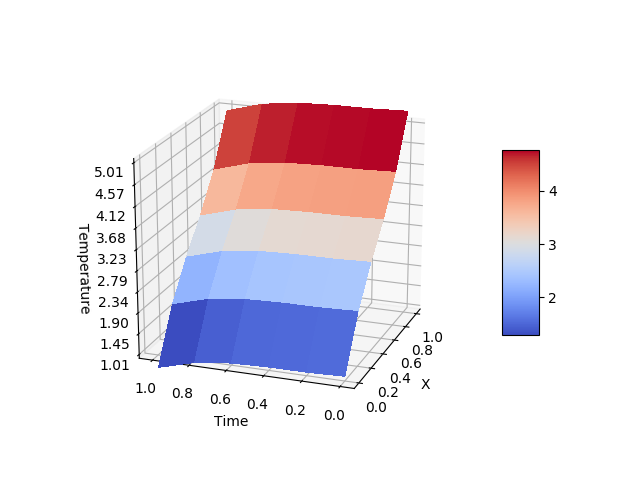
\includegraphics[width=70mm]{mainFunc5-5.png}
			\hfill
			\caption{Точное решение}
			\hfill
			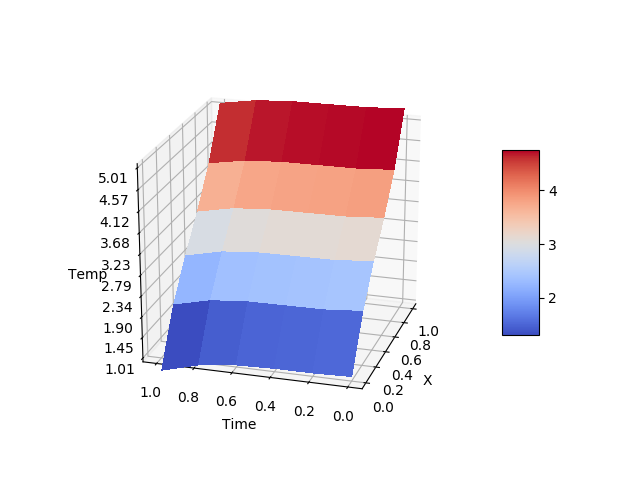
\includegraphics[width=70mm]{result5-5.png}
			\hfill
			\caption{Приближенное решение методом бегущего счета}
		\end{multicols}
	\end{figure}

	\begin{figure}[h]
		\centering
		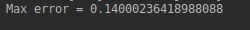
\includegraphics[width=0.3\textwidth]{MaxError5-5.png}
		\caption{Максимальная погрешность решения}
	\end{figure}
	\subsection{Для $\tau = 0.1$ и $h = 0.1$}
	\begin{figure}[h]
		\begin{multicols}{2}
			\hfill
			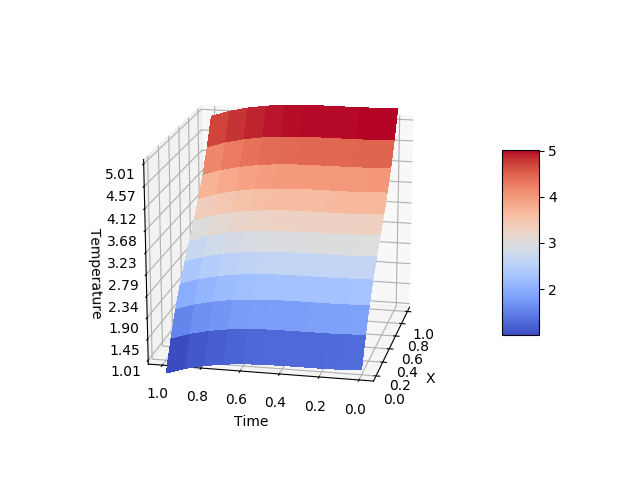
\includegraphics[width=50mm]{mainFunc10-10.png}
			\hfill
			\caption{Точное решение}
			\hfill
			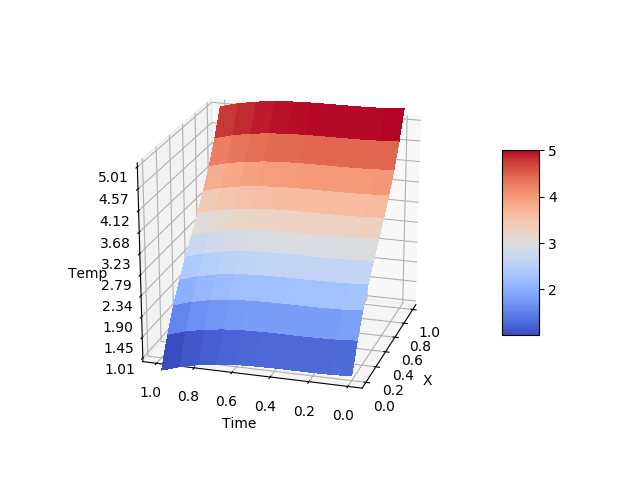
\includegraphics[width=50mm]{result10-10.png}
			\hfill
			\caption{Приближенное решение методом бегущего счета}
		\end{multicols}
	\end{figure}
	\begin{figure}[h]
		\centering
		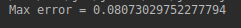
\includegraphics[width=0.3\textwidth]{MaxError10-10.png}
		\caption{Максимальная погрешность решения}
	\end{figure}

    \newpage
	Таким образом, при увеличении $\tau$ и $h$ в 2 раза погрешность решения уменьшилась примерно в 1,7 раз.
	
	\subsection{Для $\tau = 0.05$ и $h = 0.05$}
	\begin{figure}[h]
		\begin{multicols}{2}
			\hfill
			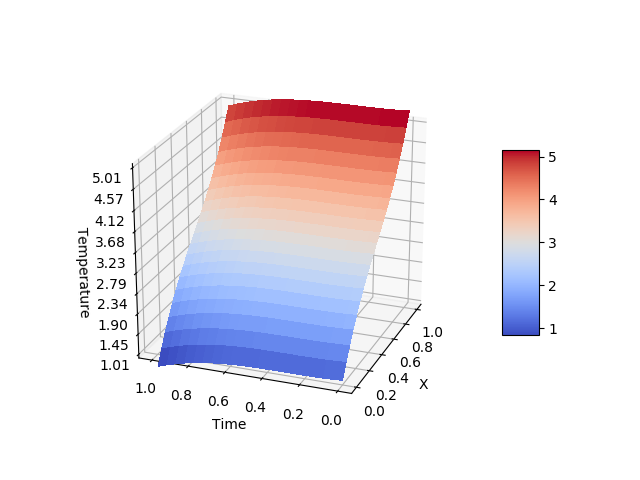
\includegraphics[width=70mm]{mainFunc20-20.png}
			\hfill
			\caption{Точное решение}
			\hfill
			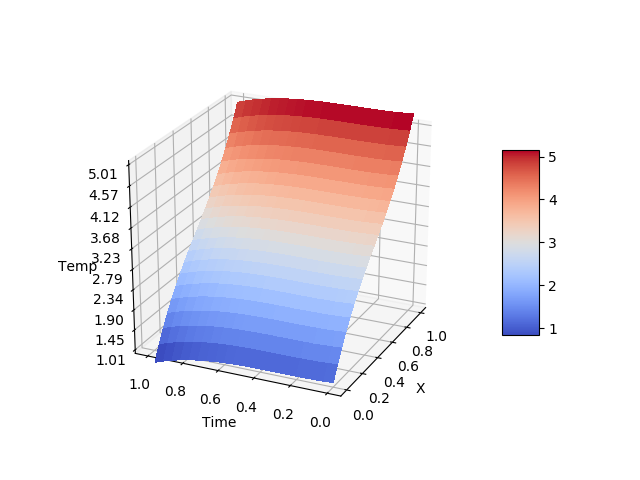
\includegraphics[width=70mm]{result20-20.png}
			\hfill
			\caption{Приближенное решение методом бегущего счета}
		\end{multicols}
	\end{figure}
	\begin{figure}[h]
		\centering
		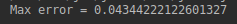
\includegraphics[width=0.3\textwidth]{MaxError20-20.png}
		\caption{Максимальная погрешность решения}
	\end{figure}
	Таким образом, при увеличении $\tau$ и $h$ еще в 2 раза погрешность решения уменьшилась примерно в 1,86 раз
	\newpage
	\subsection{График приближенного и точного решения для значений $t$ от $0$ до $1$ с шагом $\tau = 0.1$ и для $x = 0.5$}
	\begin{figure}[h]
		\centering
		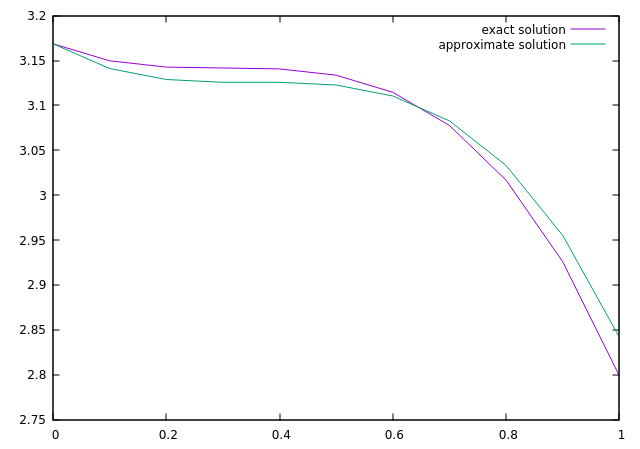
\includegraphics[width=70mm]{task3.png}
		\caption{Графики точного и приближенного решения при фиксированном $x=0.5$}
	\end{figure}
	\subsection{Для $\tau = 0.002$ и $h = 0.002$}
	Для достаточно большого числа разбиения графики практически неотличимы, но погрешность решения не нулевая.
	\begin{figure}[h]
		\begin{multicols}{2}
			\hfill
			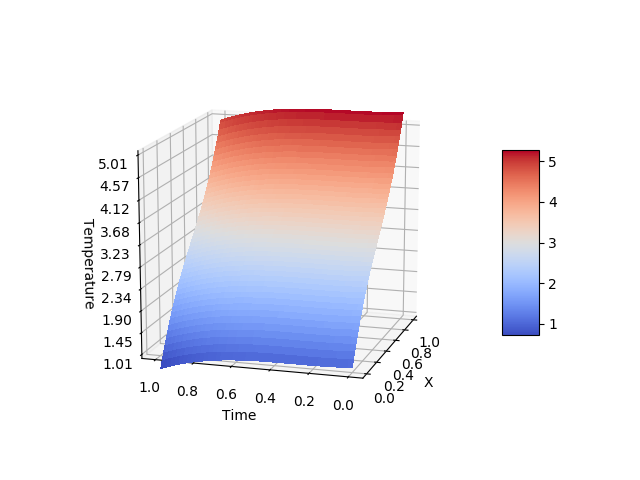
\includegraphics[width=50mm]{mainFunc500-500.png}
			\hfill
			\caption{Точное решение}
			\hfill
			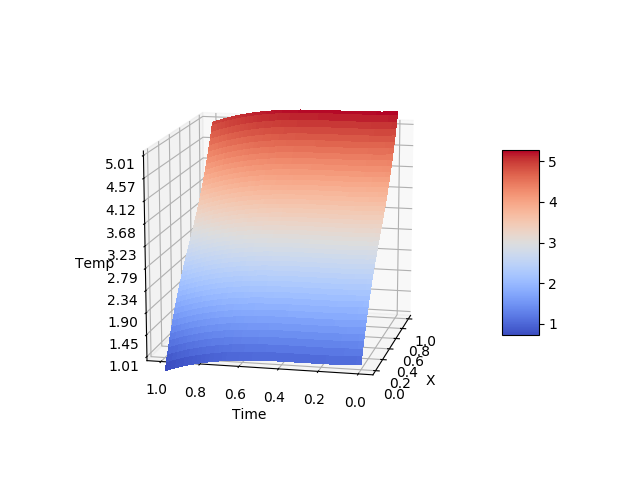
\includegraphics[width=50mm]{result500-500.png}
			\hfill
			\caption{Приближенное решение методом бегущего счета}
		\end{multicols}
	\end{figure}
	\begin{figure}[h]
		\centering
		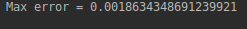
\includegraphics[width=0.3\textwidth]{MaxError500-500.png}
		\caption{Максимальная погрешность решения}
	\end{figure}
	\newpage
	\section{Выводы.}
	Таким образом мы установили, что схема бегущего счета с модификацией для $C \le 0$ является устойчивой, и не зависит от $\tau,h$ или $a$ как, например, половина этой сахемы бегущего счета, но, с другой стороны при малых $\tau, h$ погрешность решения достаточно велика и, следовательно, решение не достаточно точное.
	
	Этот метод прост для понимания и реализации, что является большим плюсом. Также убедились на практике, что данный метод при достаточно больших $\tau, h$ наше дискретное решение практически не отличимо от непрерывного, что значительно упрощает решения многих видов уравнений.
	
	Мы увидели, что теоретическая погрешность, которую мы посчитали до прогонки решения, практически совпадает с действительной погрешностью, а значит мы можем выбрать нужную нам точность решения заранее, что не мало важно для методов вычислений.
\end{document}